\chapter{MCMC}
\label{chp:appendixMCMC}

Markov Chain Monte Carlo (MCMC) methods are used to generate samples from complex probability distributions when direct sampling is infeasible. Let $\pi(x)$ be a density that we want to sample from. An MCMC algorithm constructs a Markov chain $\{X_t\}_{t\geq 1}$ with transition kernel $P(x, A)$ which has $\pi(x)$ as stationary distribution. 

One widely used MCMC method is the Metropolis-Hastings algorithm. It generates a sequence of samples from $\pi(x)$ by proposing a candidate $x'$ from a proposal distribution $q(x'|x_t)$ based on the current state $x_t$. The candidate is accepted with probability:
\[
	\alpha = \min\left(1, \frac{\pi(x') q(x_t | x')}{\pi(x_t) q(x' | x_t)}\right)
\]
If the candidate is accepted, the next state is set to $x_{t+1} = x'$; otherwise, $x_{t+1} = x_t$. 

A key property ensuring that the chain has the desired stationary distribution is that the algorithm satisfies the detailed balance condition with respect to $\pi(x)$, that is
\[
	\pi(x_t)q(x'\vert x_t)\alpha(x_t, x')=\pi(x')q(x_t\vert x')\alpha(x', x_t),
\]
for all states $x_t$ and $x'$. Provided that the Markov Chain satisfies some required regularity conditions on the proposal distribution it has the correct stationary distribution. A sufficient condition is that 
\[\pi(x)>0 \implies q(x \vert x')>0 \quad \text{for any } x, x',\]
ensuring irreducibility, and that the chain is aperiodic (\cite{robert_monte_2004}).

%Let $f(x)$ be a function of interest and assume we generate a Markov chain $\{X_t\}$ with stationary distribution $\pi(x)$. The sample average

%\[
%	\widehat{\mu}_M = \frac{1}{M} \sum_{t=1}^{M} f(X_t)
%\]

%converges to the true expectation $\mathbb{E}_\pi[f(X)]$ under mild conditions.
In practice, when using \gls*{MCMC} methods for inference the first part of the chain is discarded to allow the chain to converge to the stationary distribution. This is referred to as \emph{burn-in}.

\section*{MCMC diagnostics}
Since convergence of \gls*{MCMC} is only guaranteed asymptotically, we must rely on diagnostic methods to assess convergence when working with a finite number of samples. Assume that we do MCMC to do inference about a parameter $\theta$, which, for ease of notation, we suppose is a scalar. For models involving multiple parameters, the diagnostic methods described below are applied to each parameter individually.
 
\subsection*{Potential Scale Reduction}
A method to evaluate the convergence of a \gls*{MCMC} chain is to run several independent chains and compare the behavior between them. This is the idea of the \emph{potential scale reduction statistic} $\widehat{R}$ first introduced in \cite{Rubin}. The potential scale reduction statistic compares the between-chain variance to the within-chain variance. If all chains are at equilibrium, these will be the same, and \(\widehat{R}\) will be one. If they haven't converged to a common distribution, the \(\widehat{R}\) statistic will be greater than one.

Suppose we have a set of $K$ Markov chains $\theta_k$ which each has $M$ samples $\theta_k^{(m)}$. The between-chain variance estimate is
\[
	B=\frac{M}{K-1}\sum_{k=1}^{K}(\overline{\theta}_k^{(\boldsymbol\cdot)}-\overline{\theta}_{\boldsymbol\cdot}^{(\boldsymbol\cdot)})^2,
\]
where $\overline{\theta}_k^{(\boldsymbol\cdot)}$ is the mean for chain $k$
\[
	\overline{\theta}_k^{(\boldsymbol\cdot)}=\frac{1}{M} \sum_{m=1}^M\theta_k^{(m)},
\]
and $\overline{\theta}_{\boldsymbol\cdot}^{(\boldsymbol\cdot)}$ is the overall mean of the chains
\[
	\overline{\theta}_{\boldsymbol\cdot}^{(\boldsymbol\cdot)}=\frac{1}{K}\sum_{k=1}^K \overline{\theta}_k^{(\boldsymbol\cdot)}.
\]
The within-chain variance is averaged over the chains,
\[
	W=\frac{1}{K}\sum_{k=1}^K s_k^2,
\]
where 
\[
	s_k^2=\frac{1}{M-1}\sum_{m=1}^M (\theta_k^{(m)}-\overline{\theta}_k^{(\boldsymbol\cdot)})^2.
\]
The variance estimator is given by a mixture of the within-chain and cross-chain sample variances,
\begin{equation}
	\widehat{\text{var}}^+(\theta)=\frac{M-1}{M}W+\frac{1}{M}B,
	\label{eq:var_est_rhat}
\end{equation}
This weighted combination accounts for the uncertainty in both the within-chain and between-chain variances. Finally, we can define the potential scale reduction statistic as
\[
	\widehat{R}=\sqrt{\frac{\widehat{\text{var}}^+(\theta)}{W}}.
\]
\cite{gelman2013bayesian} introduced split-$\widehat{R}$ as a more sensitive diagnostic for convergence in \gls*{MCMC} sampling. The method involves splitting each of the $K$ chains into two halves: the first $M/2$ samples and the last $M/2$ samples, giving $2K$ chains. The standard $\widehat{R}$ statistic is then computed across these $2K$ chains. By comparing the two halves of each chain, split-$\widehat{R}$ can detect issues such as slow mixing or nonstationarity within individual chains that might be overlooked when only comparing different chains.

A typical guideline is that $\widehat{R}$ values above $1.01$ indicates that further sampling is needed (\cite{Stan} and \cite{ImprovedhatR}).

\subsection*{Effective Sample Size} % NOT RELATED AT ALL TO OTHER EFFECTIVE SAMPLE SIZE FROM RESAMPLING
\textbf{Not the same or related to ESS for resampling condition in particle filter.}\newline
An $\widehat{R}$ close to $1$ does not guarantee that an MCMC sample is reliable (\cite{VatsKnudson}). A sufficiently large \gls*{ESS} is also required to obtain stable inferences for the quantities of interest. The MCMC samples will typically be positively autocorrelated within a chain. The \gls*{ESS} is the number of independent samples with the same estimation power as the $M$ autocorrelated samples. We follow the definitions given in \cite{Stan} and \cite{ImprovedhatR}.
% Estimation error 1/sqrt{N_eff} not 1/sqrt{N}.
\todo{SETUP}
We again let $K$ be the number of chains each consistent of $M$ samples and assume all the chains have reached the stationary distribution $p(\theta)$ with mean $\mu$ and variance $\sigma^2$. The autocorrelation $\rho_t$ at lag $t\geq 0$ is defined as
\begin{align*}
	\rho_t&=\frac{1}{\sigma^2}\int (\theta^{(n)}-\mu)(\theta^{(n+t)}-\mu)p(\theta)\, d\theta \\
	&=\frac{1}{\sigma^2}\int \theta^{(n)}\theta^{(n+t)}p(\theta)\, d\theta,
\end{align*}
where we used that $\theta^{(n)}$ and $\theta^{(n+t)}$ have the same stationary distribution. We then define the effective sample size $M_{\text{eff}}$ of $M$ samples by
\[
	M_{\text{eff}}=\frac{M}{1+2\sum_{t=1}^{\infty}\rho_t}.
\]
For independent draws (i.e., \(\rho_t = 0\) for \(t \ge 1\)), we recover \(M_{\text{eff}}=M\). 
When draws are positively correlated, however, \(M_{\text{eff}}\) is smaller, reflecting the reduced information content of the chain, while if they were negatively correlated, the effective sample size will exceed the number of iterations. The \gls*{ESS} is a particular important measure, since the standard error of the estimate of a parameter decreases by $1/\sqrt{M_\text{eff}}$ and not $1/\sqrt{M}$.
 
In practice, the integral of the joint distribution $p(\theta)$ is intractable and thus we need to estimate the effective sample size. We can estimate the autocorrelation $\rho_t$ by
\[
	\hat{\rho}_t=1-\frac{W-\frac{1}{K}\sum_{k=1}^K\hat{\rho}_{t,k}}{\widehat{\text{var}}^+(\theta)},
\]
where $\hat{\rho}_{t,k}$ is an estimate of the autocorrelation at lag $t$ for the $k$th Markov chain, and $\widehat{\text{var}}^+(\theta)$ is defined in Equation~(\ref{eq:var_est_rhat}). Because of the increased noise of $\hat{\rho}1_{t}$ as $t$ increases, in practice a truncated sum of $\hat{\rho}_t$ is used. We apply Geyer’s initial monotone sequence criterion, as defined in \cite{Geyer1992}, to ensure stability. The effective sample size is estimated by 
\[
	\widehat{M}_{\text{eff}}=\frac{KM}{\hat{\tau}},
\]
where
\[
	\hat{\tau}=1+2\sum_{t=1}^{2k+1}\hat{\rho}_t=1+2\sum_{t=0}^m \hat{P}_{t}-\hat{\rho}_0=-1+2\sum_{t=0}^m \hat{P}_{t},
\]
where $\hat{P}_{t}=\hat{\rho}_{2t}+\hat{\rho}_{2t+1}$. Summing over pairs starting from lag 0 ensures that the sequence 
$\hat{P}_t$ values is non-negative and non-increasing (\cite{Geyer1992}). So, if we observe negative estimates of the autocorrelations it is due to finite-sample noise. Thus, we define an initial positive sequence by choosing the largest $m$ such that $\hat{P}_t>0$ for all $t \in \{1,\dots,m\}$. We also enforce monotonicity by modifying the sequence $\hat{P}_t$ so that it does not exceed the smallest preceding value, ensuring a non-increasing sequence.

\chapter{Bayesian model validation}
\label{chap:Bayesian_model_val}
This Chapter contains some common tools used for validating a Bayesian model.
\section*{Prior predictive check}
Before fitting a Bayesian model it is useful to assess whether the prior distributions are reasonable in the context of the model. This can be done using a prior predictive check, where data is simulated using parameters drawn from the prior. If the generated data is implausible, it suggests that the priors may be too weakly or strongly informative.

\section*{Posterior predictive check}
After fitting a Bayesian model a posterior predictive check is used to evaluate how well the fitted model explains the observed data. Here, data is simulated using parameter values sampled from the posterior distribution. If the replicated data fails to resemble the observed data, it suggests that the model may not capture key aspects of the underlying data-generating process.

\section*{Prior Sensitivity Analysis}
Prior sensitivity analysis is assessing how sensitive the model’s inferences are to the choice of prior distributions. It involves re-running the model with different reasonable priors and comparing the resulting posterior distributions. This analysis helps determine how large of an effect the prior has on the posterior.

Since it is expensive to fit the same model many times with different priors, in practice it is often done using importance sampling, see for example \cite{vehtari2024paretosmoothedimportancesampling}.

\chapter{Numerical stability tricks}
\label{chap:NumericalTricks}
This is a collection of some of the numerical tricks used in the implementation of the algorithms to avoid underflow and improve efficiency. 

\section*{Log-Sum-Exp Trick}
When aggregating the contributions of multiple particles to the log-likelihood, we need to compute a sum of the form
\[
	L_t = \frac{1}{N}\sum_{i=1}^N \exp(\ell_i),
\]
where \(N\) is the number of particles and $\ell_i$ is the $\log$-weights. Direct exponentiation of \(\ell_i\) can lead to numerical underflow if \(\ell_i\) is very small. To mitigate this, we use the log-sum-exp trick (\cite{Stan}).
Define
\[
	M = \max_{1 \le i \le N} \ell_i.
\]
Then,
\[
	\log\left(\sum_{i=1}^N \exp(\ell_i)\right) = M + \log\left(\sum_{i=1}^N \exp(\ell_i - M)\right).
\]
Thus, the incremental log-likelihood is computed as
\[
\log L_t = -\log N + M + \log\left(\sum_{i=1}^N \exp(\ell_i - M)\right).
\]
This approach rescales the log-likelihoods so that the exponential terms do not vanish numerically.

\section*{Transformation of Parameters}
When parameters are defined on constrained domains, it is often beneficial to transform them into an unconstrained space to facilitate efficient MCMC proposals. Using a standard proposal distribution, such as the normal distribution, directly in the constrained space can lead to proposed values that lie outside the domain, resulting in a likelihood of zero. Suppose we have a vector of parameters 
\[
	\theta = (\theta_1, \theta_2, \dots, \theta_n)
\]
where some components are defined on a constrained domain. For those components that are already unconstrained, we simply use the identity mapping, i.e., 
\[
	g_i(\theta_i)=\theta_i.
\]
For the constrained parameters, we introduce an invertible and differentiable transformation \(g_i\) that maps the constrained \(\theta_i\) into an unconstrained space:
\[
	\phi_i = g_i(\theta_i), \quad i = 1,2,\dots,n.
\]
A common example is proposing values for a standard deviation, which must be positive, and we can then instead propose values in $\log$-space.

If \(p(\theta)\) denotes the joint density of \(\theta\) and \(\theta_i = g_i^{-1}(\phi_i)\) is the inverse transformation, the joint density in the \(\phi\)-space is given by the change-of-variables formula:
\[
	p_{\phi}(\phi) = p\bigl(g_1^{-1}(\phi_1), \dots, g_n^{-1}(\phi_n)\bigr) \prod_{i=1}^n \left|\frac{d}{d\phi_i} g_i^{-1}(\phi_i)\right|.
\]
Taking logarithms yields the transformed log density:
\[
	\log p_{\boldsymbol{\phi}}(\boldsymbol{\phi}) = \log p\bigl(g_1^{-1}(\phi_1), \dots, g_n^{-1}(\phi_n)\bigr) + \sum_{i=1}^n \log\left|\frac{d}{d\phi_i} g_i^{-1}(\phi_i)\right|.
\]


\chapter{Supplementary Figures}
\begin{figure}
	\centering
	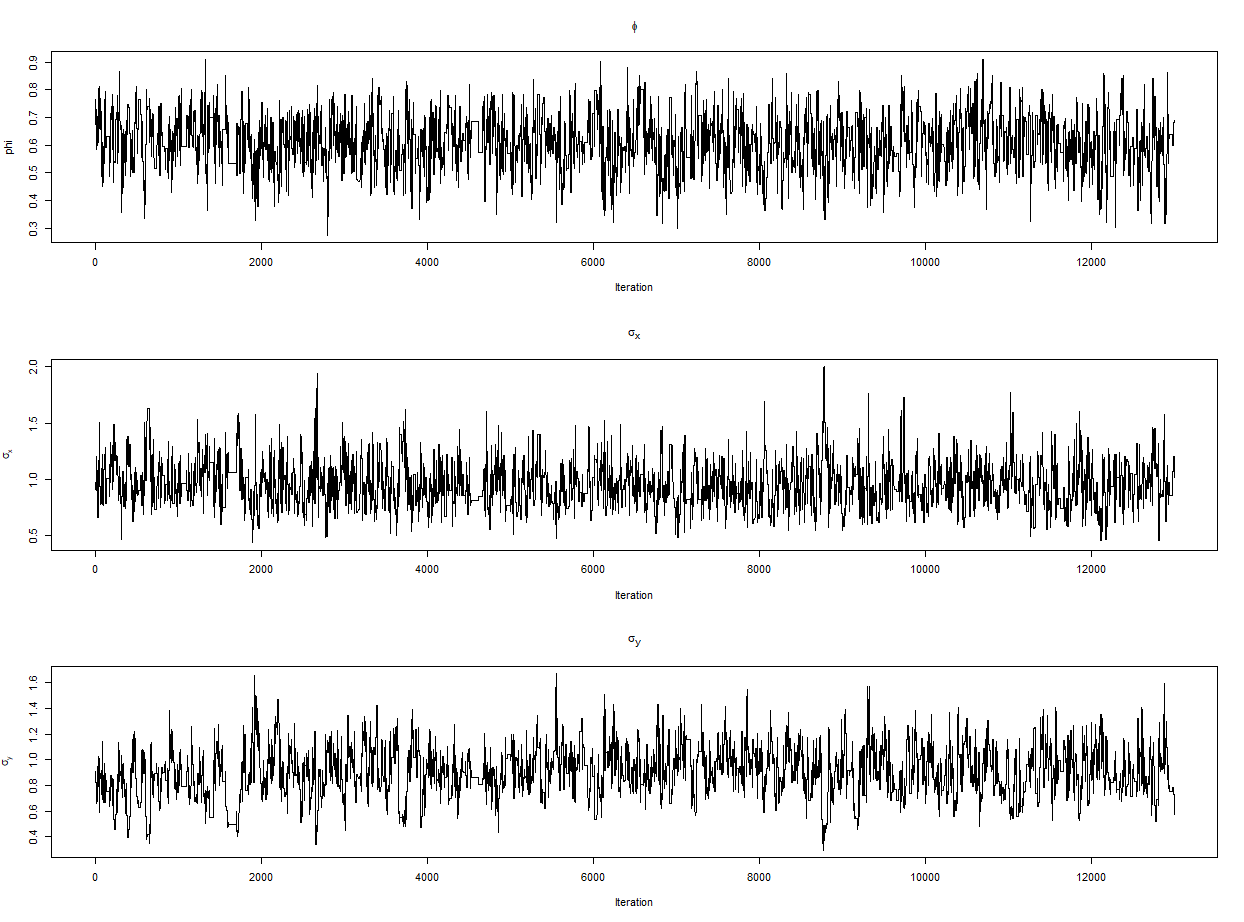
\includegraphics[width=1\textwidth]{chain_plot.png}
	\caption{A trace plot of an MCMC chain for the parameter vector $\theta=(\phi, \sigma_x, \sigma_y)$ in Example~\ref{exa:SSM_unknown_theta}\textbf{UPDATE FIGURE TO HIGH QUALITY}}
	\label{fig:chain}
	% Convert to pdf see https://www.overleaf.com/learn/latex/Inserting_Images Generating high-res and low-res images
\end{figure} 

\label{chap:supplementary_figures}
\begin{figure}
	\centering
	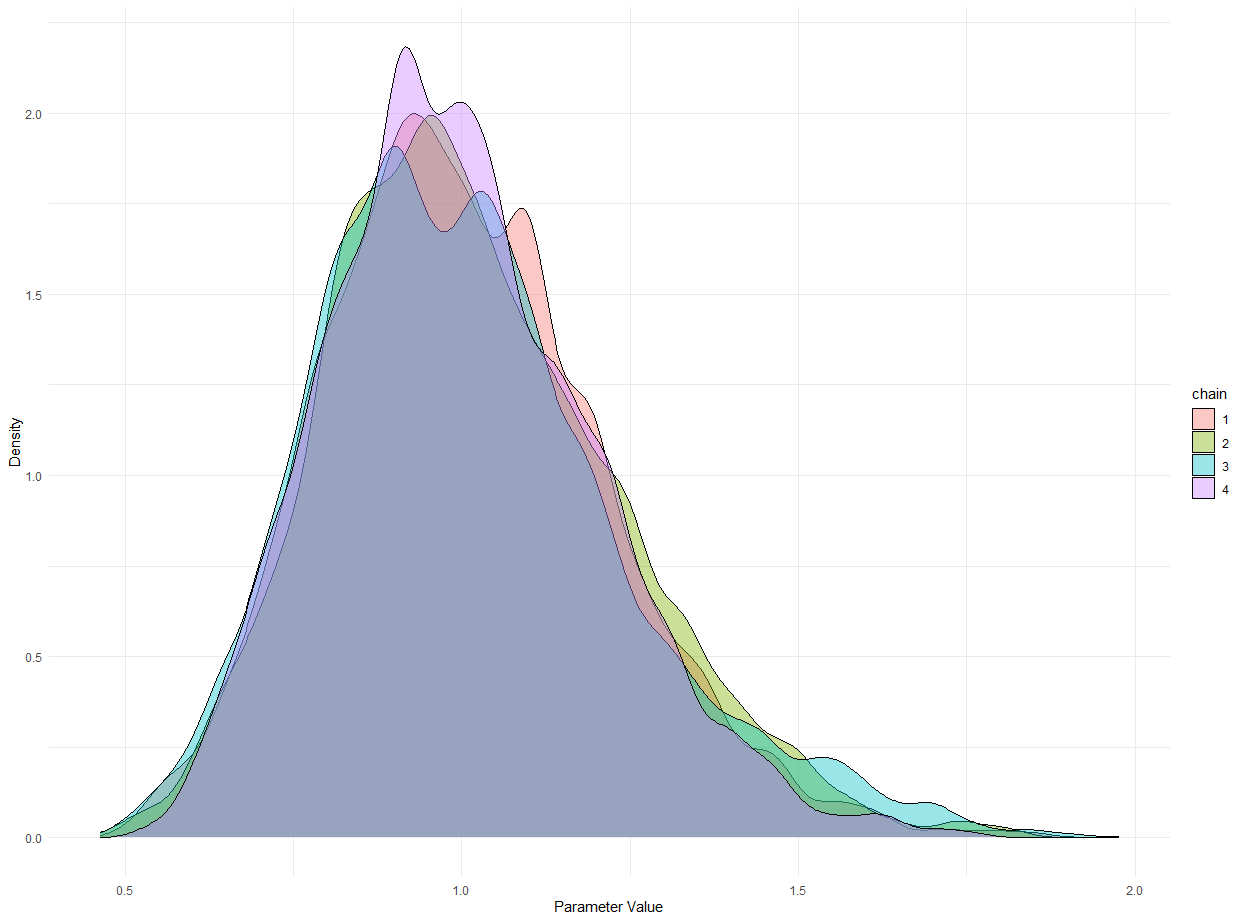
\includegraphics[width=\textwidth]{sigma_x_density_plot.png}
	\caption{Density plot of the four chains for $\sigma_x$ in Example~\ref{exa:SSM_unknown_theta}\textbf{UPDATE FIGURE TO HIGH QUALITY}}
	\label{fig:sigma_x_dens}
\end{figure}

\begin{figure}
	\centering
	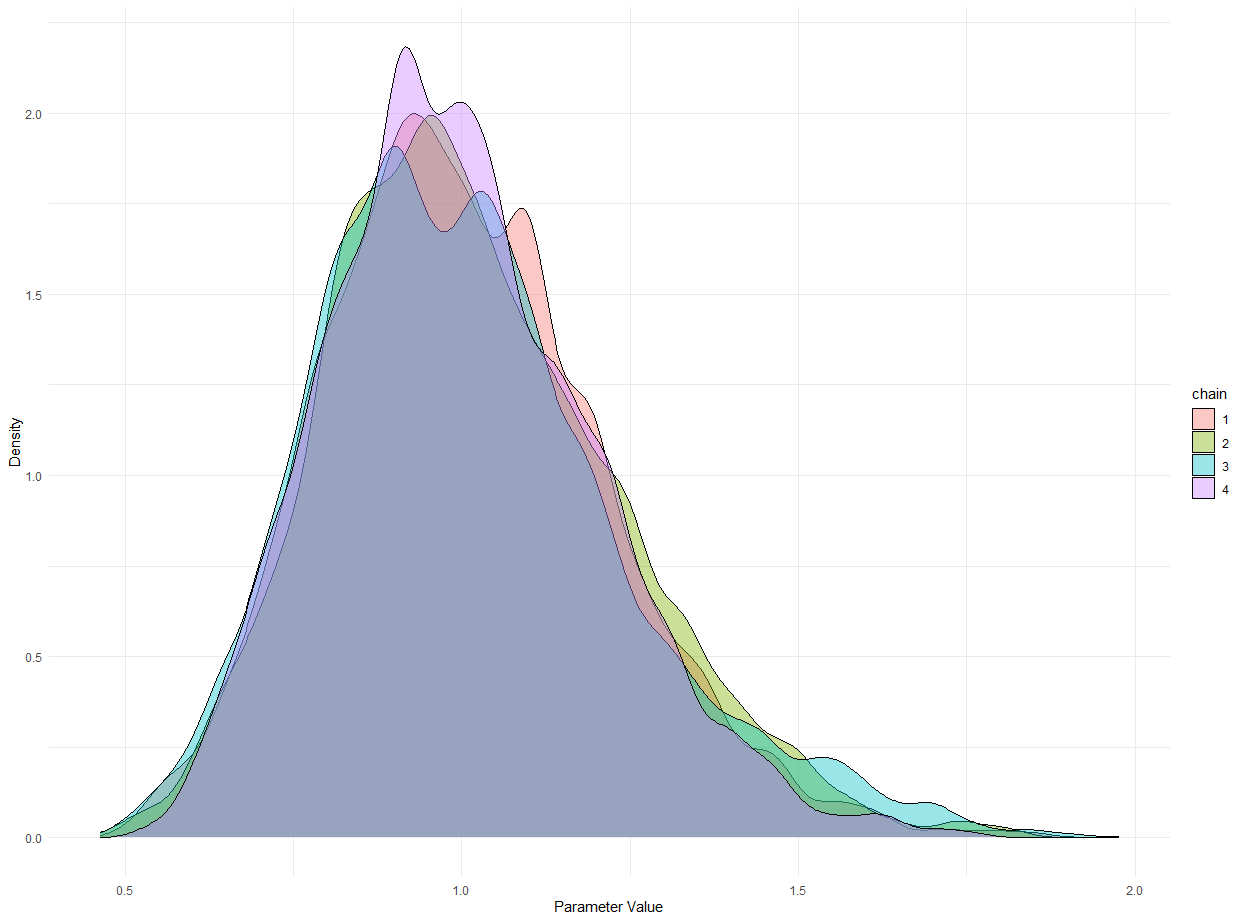
\includegraphics[width=\textwidth]{sigma_x_density_plot.png}
	\caption{Density plot of the four chains for $\sigma_y$ in Example~\ref{exa:SSM_unknown_theta}\textbf{UPDATE FIGURE TO HIGH QUALITY}}
	\label{fig:sigma_y_dens}
\end{figure}